\chapter{FETI Solvers}\label{cha:feti_solvers}
The basic system of Equations\eqref{eq:feti_equation_system} to be solved has already been derived in Chapter~\ref{cha:feti_formulation}.
\\
\\
The natural solver choice for the FETI problem is the Conjugate Gradient method. It will be shown that FETI fits neatly into the CG scheme described in Chapter~\ref{cha:iterative_solvers}.\\
This thesis is restricted to static problems, where Section~\ref{sec:natural_subspace} already explained that rigid body modes cause some problems. The solution will be the introduction of the so-called "natural subspace"
\\
Finally, a projection operator into this subspace has been derived.\\
Combining this knowledge, with the PCG algorithm introduced in Section~\ref{sec:ppcg} leads to the so-called one-level FETI method(FETI-1).\\
The projection into the natural subspace however, is also used in all other FETI algorithms.



\section{One-level FETI(FETI-1)}\label{sec:feti1}
This section aims at formulating the basic PCG algorithm specifically for the FETI problem as introduced in Chapter~\ref{cha:feti_formulation}. The name refers to the one-level of deflation(projection to the natural subspace).\\
Some alternations to the classical CG notation will be done to ensure parallel efficiency of the method.\\
\\
The PCG algorithm consists of three main points. First, new search directions are created, these search directions are then updated through orthogonalization to the previous ones, and finally an optimal step length is determined by minimizing the residual error along this direction. In practice, orthogonalization is performed with regards to all previous search directions due to the finite precision of the machine.
\\
The first question is therefore, how to derive the search directions. Since FETI operates on interface forces as primary variables, we need an update for the force vector.\\
\\
The FETI-1 algorithm is outlined in Figure~\ref{strukt:feti1}. The reader may note the relation to Figure~\ref{struk:MPPCG}.
\\
\begin{figure}[ht]
  \centering
  \subimport{}{\tikzpath/algorithm_feti1.tex}
  \caption[Structogram FETI-1 algorithm]{Structogram of the FETI-1 algorithm. It can be classified as a Projected Preconditioned Conjugate Gradient algorithm as described in Section~\ref{sec:ppcg}. The coarse $\nullspacemat$ grid is built upon the rigid body modes. The solution in the coarse space is searched for directly, the Conjugate Gradient then gives the natural subspace component. The solution is finally obtained as a sum of those two.}
  \label{strukt:feti1}
\end{figure}

\section{Two-level FETI(FETI-2)}\label{sec:feti2}
The so-called FETI-2 algorithm can be classified as an Projected (Preconditioned) Conjugate Gradient algorithm just like FETI-1.
\\
As mentioned in Section~\ref{sec:scalability}, the main difference lies in the introduction of an auxiliary coarse space.\\
Albeit derived as necessity for heterogeneous structural dynamics problems, a suitable auxiliary coarse space has also proven very useful for static FETI calculations. Therefore, every FETI-1 method, enhanced by an auxiliary coarse space of any kind shall now be called a FETI-2 method, referring to the two levels of projection.\\
One particular example of the general advantage of an auxiliary coarse space was first described in~\cite{Farhat1998} an further analysed in~\cite{Farhat2000}.\\
The basic FETI-1 algorithm shows bad convergence due to limited error propagation, especially for heterogeneities, see Chapter~\ref{cha:numerical_assesment}. This is also reflected in the very broad eigenvalue distribution of FETI-1 (see Figure~\ref{fig:eigvalues_pointdistribution}).\\
A possible solution is the introduction of an auxiliary coarse space, that holds critical modes. The idea is to identify the bad eigenmodes, or an approximation thereof, and to then solve the problem in a subspace (the so-called coarse space) orthogonal to these eigenmodes:
\begin{align}
  \tp{\cspace}\totalgap_i=\dvec{0}         
  \label{eq:orthogonality_coarse_subspace} 
\end{align}
which is completely analogous to Equation~\eqref{eq:orthogonality_natural_subspace}.\\
The coarse space projector can thus be derived as
\begin{align}
  \projc=\eyemat-\cspace\inv{(\tp{\cspace}\locdualschur\cspace)}\tp{\cspace}\locdualschur 
\end{align}
\\
The FETI-2 algorithm is described in Figure~\ref{strukt:feti2}.

\begin{figure}[h!]
  \centering
  \subimport{}{\tikzpath/algorithm_feti2.tex}
  \caption[Structogram FETI-2 algorithm]{FETI-2 algorithm. Differences to the classical FETI-1 algorithm are underlined red.}
  \label{strukt:feti2}
\end{figure}

\subsection{Generalized eigenvalues in the overlap(Geneo)}
A mathematically appealing approach for the definition of the auxiliary coarse space $\cspace$ in a FETI-2 method are the so-called Geneo methods (Generalized eigenvalues on the interface).\\ The idea is to identify the "bad" eigenmodes, corresponding to the "bad" eigenvalues in the spectrum of the system matrix (see Figure~\ref{fig:eigvalues_pointdistribution}) and to build up the auxiliary coarse space with them. The coarse problem is solved for directly, before the CG iterations themselves are then performed in a subspace orthogonal to these modes, the spectrum of the projected system matrix can thus be significantly improved. Extensive analysis of this methods\cite{Spillane2016}\cite{Spillane2013}\cite{Spillane2014} has shown their remarkable robustness, especially for the generally quite challenging FETI problems described in Chapter~\ref{cha:numerical_assesment}. However, although mathematically found and robust, the eigenvalue problems on the interface introduce a substantial computational overhead and cannot be parallelized well. What is more increasing the size of the auxiliary coarse grid degenerates the parallelizability of the algorithm further. Thus other methods like the family of Multi Preconditioned Conjugate Gradient solvers are generally more efficient for engineering problems.

\section{Simultaneous FETI(FETI-S)}\label{sec:fetis}
The FETI-1 and FETI-2 algorithm use one search direction at each iteration for the whole interface problem. For the specific case, where the preconditioner is built as a sum of local contributions, however, we have already introduced the appealing approach of Multi Preconditioned (Projected) Conjugate Gradient in Section~\ref{sec:mpcg}. This is exactly the case in FETI, in fact, the local preconditioners $\locdualschur$ have to be built anyway, so no additional work is introduced here.\\
The application of the MPPCG concept to the FETI problem is called simultaneous FETI, or FETI-S, and was first described in \cite{RixenPhD} for two sub-domains, and consequently generalized to an arbitrary number of sub-domains in \cite{Rixen2013}.
The basic idea is to exploit the additive structure of the preconditioner(see Equation~\eqref{eq:definition_dualschur}).
One can thus precondition each substructure independently, which results in $s$ search directions that can be searched for.
\begin{align}
  \Zmat_i=\begin{bmatrix} \cdots,\ids{\scaled{\asmop}} \ids{\traceop} \ids{\scaled{\locschur}} \tp{\ids{\traceop}} {\ids{\scaled{\asmop}}}{}^T \resvec_i,\cdots \end{bmatrix} 
\end{align}
The crucial advantage of this method is that, although at each iteration, on minimizes with respect to $s$ search directions, the cost of each iteration is not increasing proportionally, as explained in Section~\ref{sec:fetis_cost}. Particularly, the number of Neumann solves on the substructures is not increased.

\begin{align}
  \scaled{\locschur}=\sum_s \ids{{\scaled{\asmop}}} \ids{\traceop} \ids{{\scaled{\locschur}}} \tp{\ids{\traceop}}
  {\ids{{\scaled{\asmop}}}}{}^T                                                
\end{align}
Additionally, the scaling approaches as explained in Section~\ref{sec:precond} are applied to the preconditioner.
The efficiency of the FETI-S algorithm was substantially improved in~\cite{Gosselet2015} by introducing an important trick, that localized the application of the FETI operator.
Moreover, the paper also provides an efficient implementation of the Conjugate Gradient algorithm, that all FETI algorithms provided in this paper are based on.
Generally, the FETI-S algorithm can be classified as a Multi Preconditioned Conjugate Gradient Algorithm (MPPCG)\cite{Bridson2006}.\\
It is noteworthy, that since MPPCG algorithms do not minimize in a Krylov subspace, a heuristic bound for the number of iterations can not be justified. However, extensive numerical analysis have certified a very robust behaviour.\\
A detailed description of the FETI-S algorithm is provided in Figure~\ref{strukt:fetis}

\subsection{Computational cost of FETI-S}\label{sec:fetis_cost}
The idea of FETI-S seems appealing. But  of course, the increased number of search directions does not come without a price. Efficiency considerations have been carried out by~\cite{Gosselet2015} and this chapter aims at pointing out the most important aspects.
First of all, we note that the communication patterns of the algorithm do not change compared to FETI-1, they only involve more data.\\
Secondly, we obviously see that the most important part of any FETI algorithm are the local Neumann and Dirichlet solves. Compared to the FETI-1 algorithm, the preconditioner now has to be applied all columns of $\sdirnspacemat$ instead of just a simple vector. The overhead of this is low.\\
The paper also introduced a clever method to improve the efficiency of this step by exploiting the locality of $\sdirfspacemat$:

\begin{align}
\sdirnspacecspaceblock_{i+1} = \locdualschur \dmat{W}_{i+1} = \locdualschur \projn \Zmat_{i+1} -
\sum_{j=0}^i \sdirnspacecspaceblock_j \pinv{\Deltamat_j} \dvec{\phi}_{i,j} \\
\end{align}
Inserting the very definition of the natural subspace projector as defined in Equation~\eqref{eq:TODO} one can write
\begin{align}
\sdirnspacecspaceblock_{i+1} = (\locdualschur \Zmat_{i+1} - \locdualschur \dmat{A} \dmat{G} \pinv{(\tp{\dmat{G}} \dmat{A} \dmat{G})} \tp{\dmat{G}} \dmat{Z}_{i+1}  ) - \sum_{j=0}^i \sdirnspacecspaceblock_j \pinv{\Deltamat_j} \dvec{\phi}_{i,j} \\
 \end{align}
Thanks to this reformulation, only localized Neumann problems need to be solved and the efficiency is greatly improved.\\
Furthermore, the multiple Neumann problems can typically be solved simultaneously on different processors since parallelism was the motivation for these algorithms in the first place.\\
Another source of numerical overhead is the (pseudo-)inversion of $\Deltamat_i$, which is typically dense. However, its size is $numsubstruct \times numsubstruct$ and thus relatively small compared to the interface-based operators.



\begin{figure}[h!]
  \centering
  \subimport{./}{fig/tikz/algorithm_fetis.tex}
  \caption[Structogram FETI-S algorithm]{The simultaneous FETI algorithm  is an implementation of the Multi Preconditioned Conjugate Gradient as described in Section~\ref{sec:mpcg}. Each substructure contributes its own search direction that is solved for independently of the others.}
  \label{strukt:fetis}
\end{figure}


\section{Adaptive Simultaneous FETI(FETI-AS)}\label{sec:fetias}
As explained before, the FETI-S solver is just an application of the MPPCG concept, described in Section~\ref{sec:mpcg} on the FETI problem. As already mentioned, while the FETI-S method shows very good convergence rates, its iterations become more expensive with an increasing number of subdomains. AS will be pointed out in the following sections, typically some search directions are more important than others. It thus seems intuitively to try to identify the really important search directions, and restrict iterations on them. This is exactly what the Adaptive Multi Preconditioned Conjugate Gradient algorithm~\ref{sec:ampcg} does. Applied on the FETI problem, an Adaptive Simultaneous FETI solver can thus be found as described in Figure~\ref{strukt:fetias}.\\

\begin{figure}[h!]
  \centering
  \subimport{./}{fig/tikz/algorithm_fetia.tex}
  \caption[Structogram FETI-AS algorithm]{Structogram of the Adaptive Simultaneous FETI algorithm. The algorithm is quite analogue to the FETI-S one. The differences are marked in red. This version shows the implementation of a local $\tau$ criterion. Compared to the often used global one, the local criterion allows to iterate on an arbitrarily reduced number of search directions}
  \label{strukt:fetias}
\end{figure}

As explained in Section~\ref{sec:ampcg} the appropriate choice of $\tau$ can become quite delicate in this algorithm. We have already introduced an estimation formula based on a prescribed contraction factor $\rho$ and the minimum eigenvalue of the system matrix. However, all the analyses carried out during this thesis showed that the optimal choice for both $\tau$ and $\rho$ is problem-dependent.\\
In the following, a quick analysis on this issue has been conducted. The setup is the same as in Figure~\ref{fig:setup_visualization_searchdirs} and results are provided in Figure~\ref{fig:results_study_contractfac}. It can be shown that the necessary number of search directions can be significantly reduced, without increasing the overall iteration count.\\
We therefore prefer a direct choice of tau over the calculation with the contraction factor. If implemented so, the Adaptive Simultaneous FETI algorithm hardly introduces any additional work in the $\tau$-test, while providing remarkable potential for increasing the efficiency. We therefore suggest that this algorithm should, in principle, always be favoured to simple FETI-S. If in doubt, one better chooses $\tau$ bigger, since in the limit $\tau \rightarrow \infty$ the FETI-S algorithm is retrieved.


\begin{figure}[ht]
  \begin{center}
    \includestandalone{./fig/tikz/tau_formula}
    \caption[Visualization $\tau$-$\rho$ relation]{Relation between the contraction factor and $\tau$ according to the formula $\frac{1-\tau^2}{\lambda_{min} \tau^2}$. In can be observed, that for a wide range of $\rho$ $\tau$ does not change dramatically}
    \label{fig:fetias_tau_formula}
  \end{center}
\end{figure}


\begin{figure}[ht]
  \begin{center}
    \includestandalone{./fig/tikz/study_contractfac_setup1}
    \caption[Choice of $\tau$ - problem 1]{Study for the optimal choice of $\tau$. The problem described in Figure~\ref{fig:visualization_fetias_searchdirs} is considered here. Three different choices for $\rho$ or $\tau$ respectively were tested. The plots visualized the number of search directions during each iteration of the FETI-AS solver. Obviously, the total number of iterations is given by the number of bars in each plot. The figure shows, that an appropriate choice of the parameter $\tau$ is crucial in order to exploit the full potential of the FETI-AS Solver. In the top figure, $\tau$ has obviously been chosen to big, thus the number of search directions is not significantly reduced. In the bottom figure, $\tau$ has been chosen too small, thus the total number of iterations is highly increased, making the advantage of reduced search directions to naught. In the analysis carried out during that thesis, $\tau=\myorder{1}$ has shown to be a reasonable choice and can thus be recommended as a guideline.}
    \label{fig:results_study_contractfac}
  \end{center}
\end{figure}


\begin{figure}[ht]
  \begin{center}
    \includestandalone{./fig/tikz/study_contractfac_setup2}
    \caption[Choice of $\tau$ - problem 2]{Another study for the optimal choice of $\tau$. In contrast to the setup in Figure~\ref{fig:results_study_contractfac_setup2}, the domain was split only in half the number of substructures an the domain ratio was changed from 1:1 to 1:3. What is more, a softer material was used. What this aims at is a demonstration that even the contraction factor $\rho$ is not problem independent. This of course constitutes a huge draw back on the generalizability of the FETI-AS method.}
    \label{fig:results_study_contractfac_setup2}
  \end{center}
\end{figure}


\begin{figure}[ht]
  \begin{center}
    %\includestandalone{./fig/tikz/study_contractfac_steps_visualization}
    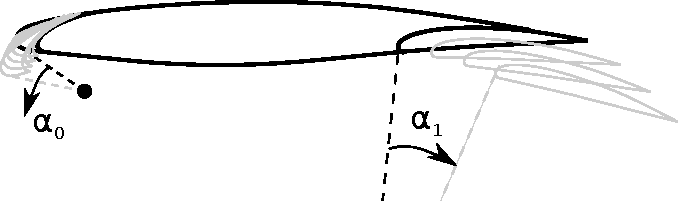
\includegraphics[width=0.35\textwidth]{\studypath/2016-08-25_StudyContractfac/setup/setup.pdf}~\hspace{1cm}
    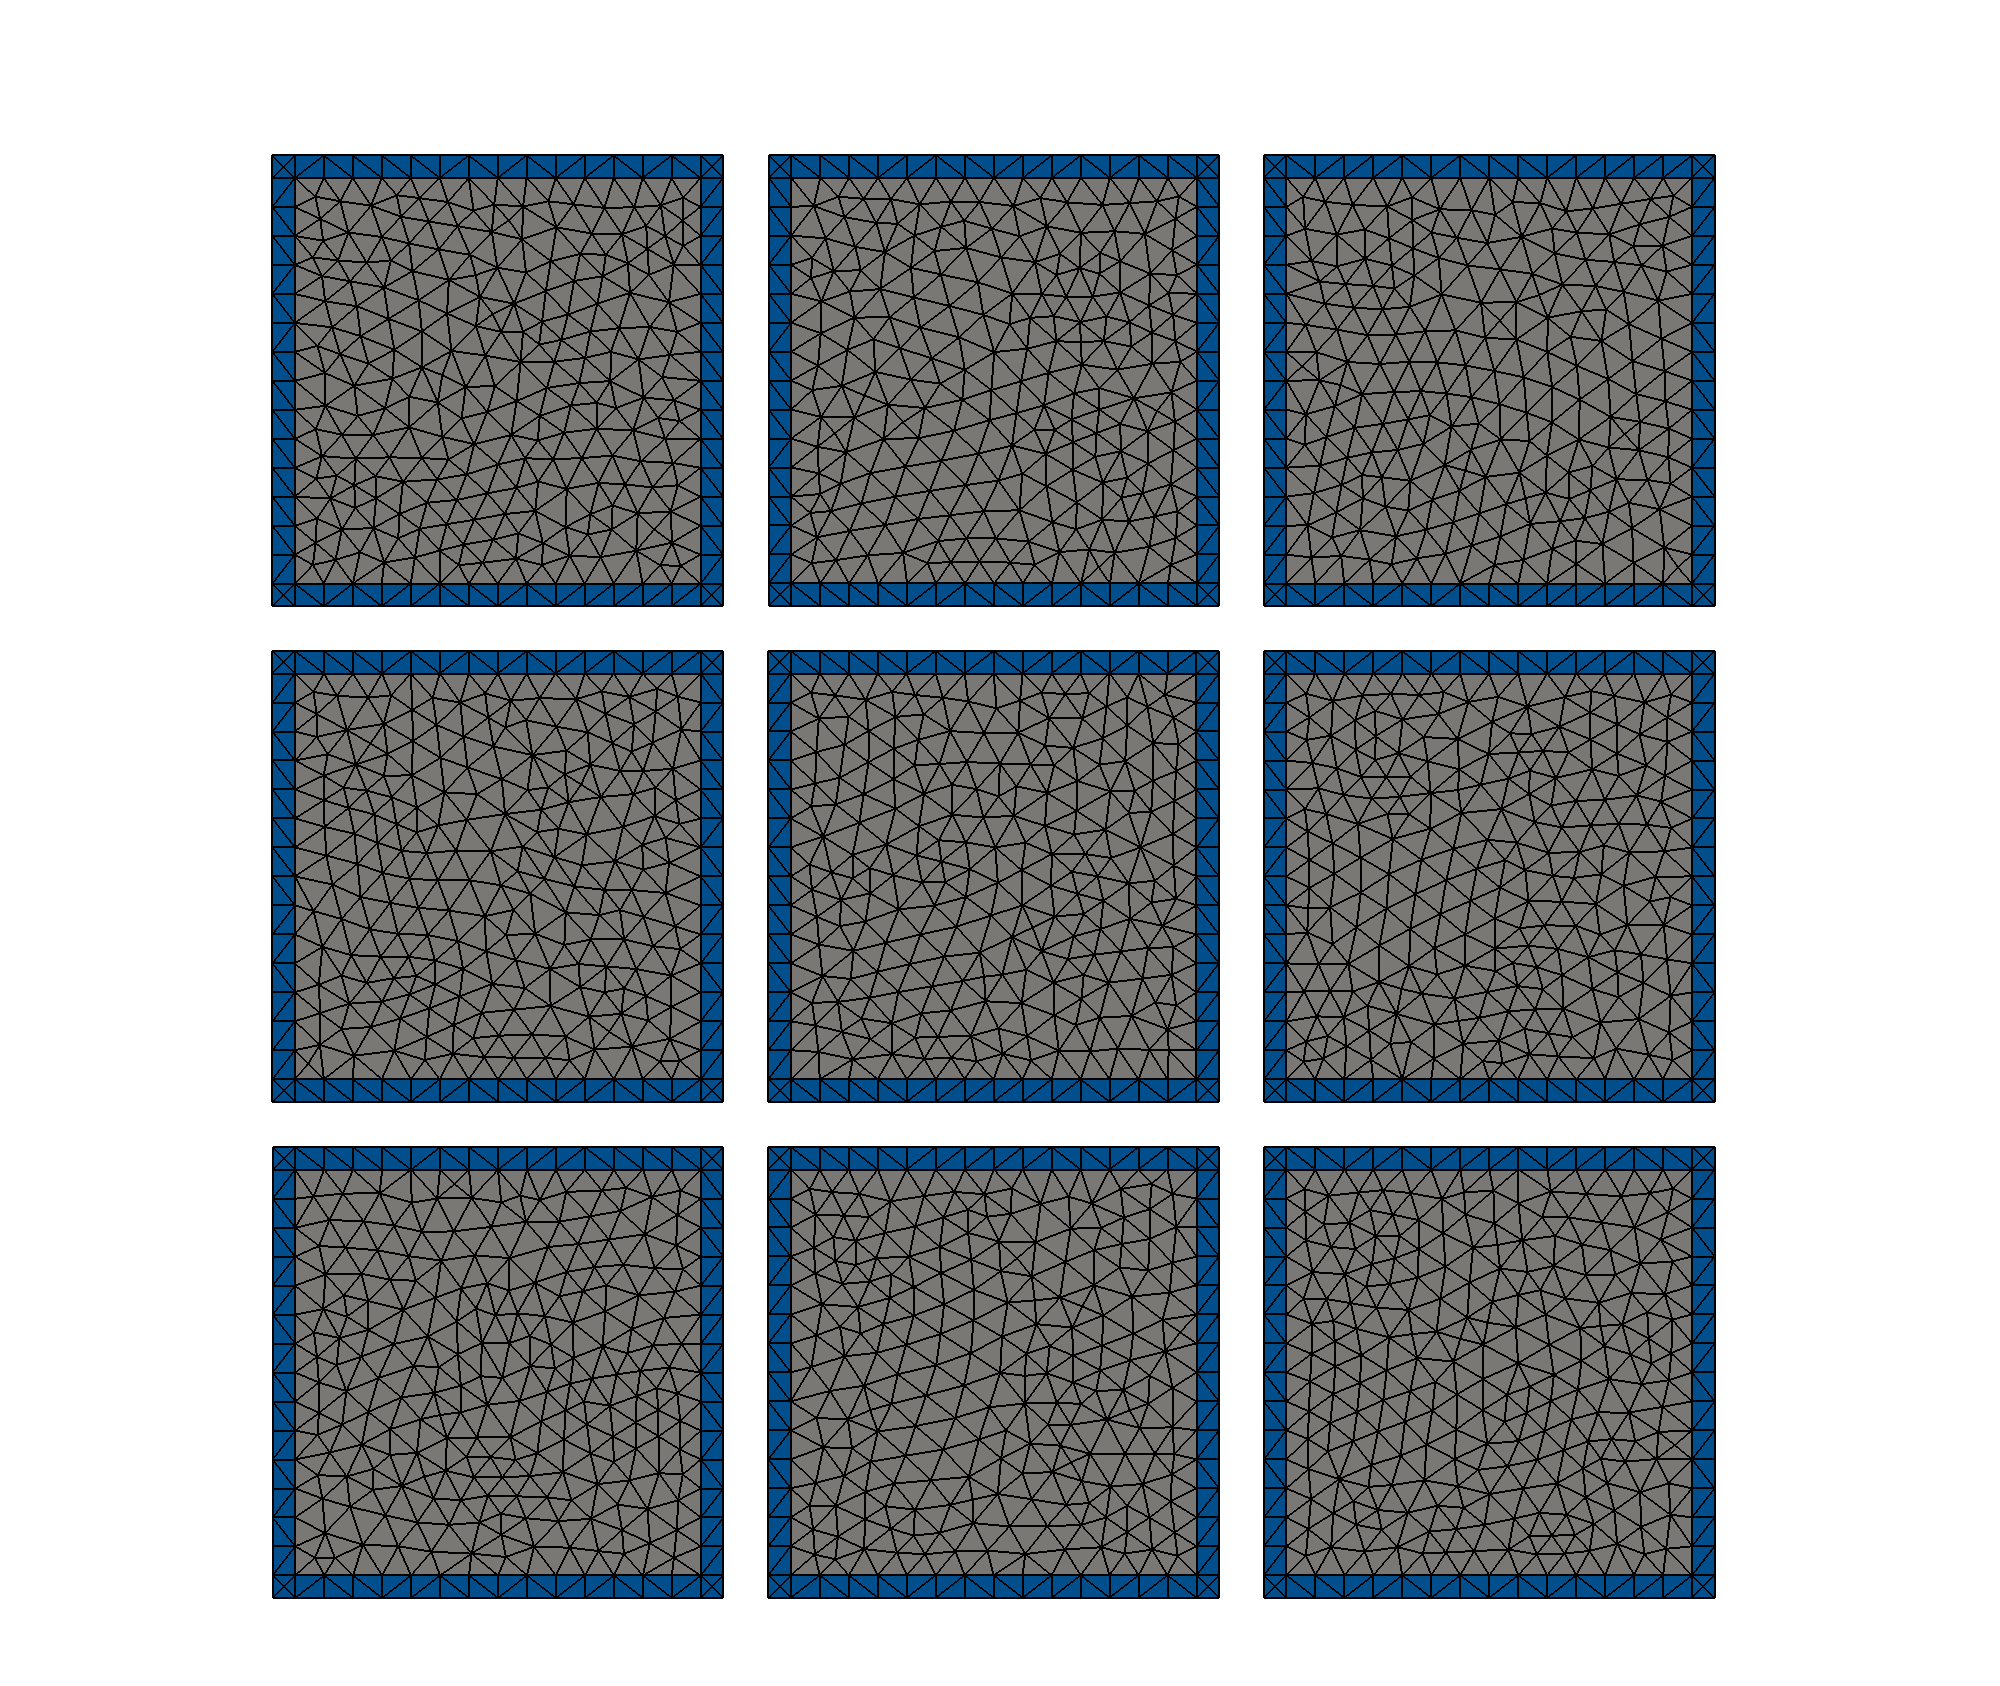
\includegraphics[width=0.30\textwidth]{\studypath/2016-08-25_StudyContractfac/setup/partitioning.pdf}~
    \caption[Setup for visualization of search directions in FETI-S]{Setup for the visualization of search directions. A square-shaped domain is used. The bearing is statically determined on the left border. The whole structure is subjected to gravity. The two materials (blue and grey) are aligned in an checkerboard pattern. Their stiffness ratio is 1:100. It will be explained in Section~\ref{sec:heterogeneities}, why heterogeneous problems are of special interest.}
    \label{fig:setup_visualization_searchdirs}
  \end{center}
\end{figure}

%/home/lukas/Desktop/SA_Thesis/studies/2016-08-25_StudyContractfac/setup/setup.pdf


\begin{figure}[h!]
  \begin{center}
    %\includestandalone{./fig/tikz/study_contractfac_steps_visualization}
    \includegraphics[width=0.7\textwidth]{./fig/tikz/study_contractfac_steps_visualization.pdf}
    \caption[Visualization of search directions in FETI-S]{Visualization of the search directions in an Simultaneous FETI simulation of the problem setup described in Figure~\ref{fig:setup_visualization_searchdirs}. All figures are warped by differently scaled displacement vectors for better visualization. The color corresponds to the step that the algorithm takes in that iteration. The figures show two things. Firstly, the algorithm is obviously very effective in capturing the largest errors. Secondly, with an increasing iteration number, the steps are effectively concentrated on very small areas. This is very well reflected in Figure~\ref{fig:results_study_contractfac}, where the number of search directions, that the FETI-AS solver chooses to work on, significantly reduces over the iterations and explains why FETI-AS shows hardly any slowdown in the convergence compared to FETI-S.}
    \label{fig:visualization_fetias_searchdirs}
  \end{center}
\end{figure}


\subsection{Fast Adaptive Simultaneous FETI(FETI-FAS)}\label{sec:fetifas}
The previous section has highlighted the potential superiority of the FETI-AS solver compared to the FETI-S one. Many search directions seem to be not that important, so neglecting them does not really increase the total iteration count much.\\
Looking at Figure~\ref{fig:results_study_contractfac} one can also note two things. Firstly, it seems that with progressing iteration, more and more search directions can be neglected, while it does make sense to use all search directions at first.\\
Secondly, the optimal choice of $\tau$ is crucial and, unfortunately, it is problem-dependent. This problem can be avoided by prescribing a contraction factor $\rho$ according to Equation~\eqref{eq:general_ampcg_conditions}, this does, however, introduce an eigenvalue problem and it is often difficult to draw a clear line between the smallest eigenvalue and eigenvalues that are numerically zero, due to the projection.\\
This section is thus dedicated to a thorough analysis of these mechanisms. Specifically, new approaches will be introduced for the selection of important search directions. Since they avoid the expensive $\tau$-test, they will be denoted as Fast Adaptive Simultaneous FETI schemes(FETI-FAS) in this thesis.\\
Numerical analysis will finally test their robustness and performance compared to FETI-AS and conclusions will be drawn in Chapter~\ref{cha:summary}.


\paragraph{The problem with FETI-1/FETI-2}
For the following considerations, the setup already described in Figure~\ref{fig:setup_visualization_searchdirs} will be discussed. Iteration numbers for this problem have already been provided in Figure~\ref{fig:resuts_study_contractfac}. It seems that the more the algorithm is shifted towards the classical FETI-1 approach, the more rapidly the total iteration count increases. Indeed, the same problem solved with FETI-1 takes 147 iterations.\\
To analyse this behaviour the development of the convergence indicator $\ids{t}$ for the substructures has been visualized in Figure~\ref{fig:ts_development}. It can bee seen, that FETI-S is much more capable of improving the substructure solutions uniformly, compared to FETI-1. The reason is, that in FETI-1, all substructure directions are simply summed up. So few contributions dominate the sum. More over, the same force value, relating to a Lagrange multiplier, is used for both sides of the interface in FETI-1, which can lead to significant errors.\\
Noting that the calculation of $\ids{t}$ does not introduce a significant overhead, one could think of several ways to improve the convergence:
\begin{enumerate}
  \item Build blocks of search directions according to their contribution factor
  \item Select search directions which showed a decreasing contribution factor
  \item Select the search directions with lowest $\ids{t}$
\end{enumerate}


\begin{figure}[h!]
  \begin{center}
    \subimport{./}{\tikzpath/algorithm_fetifas_scheme1}
    \caption[Structogram FETI-FAS scheme 1]{Scheme 1 for the FETI-FAS approach as described in Section~\ref{sec:fetifas}. The substructure convergence indicator as sorted in ascending order in each iteration. The substructure indices are then grouped block-wise, according to their convergence indicator. Each block gives one summed up search direction. The search space is then created with these search directions.}
    \label{strukt:fetifas_scheme1}
  \end{center}
\end{figure}

\begin{figure}[h!]
  \begin{center}
    \subimport{./}{\tikzpath/algorithm_fetifas_scheme2}
    \caption[Structogram FETI-FAS scheme 1]{Scheme 2 for the FETI-FAS approach as described in Section~\ref{sec:fetifas}. The substructure convergence factors are compared to the previous iterations. If it decreased than the search directions is incorporated into the search space. For a specified number of iterations at the beginning, all search directions are used. In order to avoid the incorporation of search directions that relate to already converged substructures due to numerical fluctuations, search directions are no longer incorporated into the search space, if their convergence factor has converged up to a factor of 100 to the simulation tolerance. For all calculations during this thesis, this barrier has shown to be practical.}
    \label{strukt:fetifas_scheme1}
  \end{center}
\end{figure}

\begin{figure}[h!]
  \begin{center}
    \subimport{./}{\tikzpath/algorithm_fetifas_scheme3}
    \caption[Structogram FETI-FAS scheme 1]{Scheme 3 for the FETI-FAS approach as described in Section~\ref{sec:fetifas}. The substructure convergence indicator as sorted in ascending order in each iteration. Only the directions with lowest $t_i^s$ are incorporated into the search space.}
    \label{strukt:fetifas_scheme1}
  \end{center}
\end{figure}

The results for all three approaches are visualized in Figure~\ref{fig:fetifas_schemes}. Due to the results of that figure, scheme 2 has been favoured for the rest of this thesis. If not mentioned otherwise FETI-FAS refers to that scheme from now on

\begin{figure}[h!]
  \begin{center}
    \includestandalone{\tikzpath/study_contractfac_ts-development}
    %\includegraphics[width=\textwidth]{./fig/tikz/study_contractfac_ts-development.pdf}
    \caption[Development of convergence indicator during FETI-2 and FETI-S iterations]{Plot of the substructure convergence indicator $\ids{t}$ for FETI-2 and FETI-S. Of course, $\ids{t}$ is irrelevant for those solvers. However, they give a pretty good interpretation on how the choice of $\tau$ influences the converge properties of a FETI-AS simulations. Every FETI-AS search space includes the direction, created by the simple sum of preconditioners, as can be seen in Figure~\ref{strukt:fetias}. Some directions are then additionally added according to the so called $\tau$-test(step (15) in Figure~\ref{strukt:fetias}). If all directions are added, a classical FETI-S is retrieved.}
    \label{fig:ts_development}
  \end{center}
\end{figure}



\begin{figure}[h!]
  \begin{center}
    \includestandalone{\tikzpath/study_contractfac_fetifas}
    %\includegraphics[width=\textwidth]{./fig/tikz/study_contractfac_ts-development.pdf}
    \caption[Results for the proposed FETI-FAS schemes]{Results for the three proposes FETI-FAS schemes. All three approaches significantly reduced the iteration count compared to FETI-1. For scheme 1, the limit for the admission of search directions has been set relative to the convergence criterion by a factor of 100. For scheme 2, the four search directions with lowest $\ids{t}$ have been used in each iteration. For scheme 3 two search directions, built by the sum of the the lower and upper half of search directions respectively, were used.\\
    Overall, the first scheme seems to be the most promising one and is therefore used for the rest of this thesis. However, scheme 2 also shows some advantages since the constant number of search directions makes efficient load balancing easier.}
    \label{fig:fetifas_schemes}
  \end{center}
\end{figure}






%\section{FETI-B}
%The block FETI method (FETI-B) is based on the idea of the block Conjugate Gradient algorithm~\cite{OLeary1980}.
%Compared to FETI-1, a block of right hand sides is used to activate the local effects. In other words, it exploits the additive structure of the interface displacements $\ifacedispvec$ just like FETI-S exploits the additive structure of the pre-conditioner. The FETI-B method was first proposed in~\cite{Gosselet2015}, and has shown to require slightly less iterations than the FETI-S method. However it introduces the drawback of additional local Dirichlet and Neumann solves, while the main advantage, the elimination of full re-orthogonalization, can not be exploited in real codes, due to round-off error.\\
%First numerical studies, however, have attested the method noticeable reductions in the iteration numbers when it comes to cross-points and very irregular meshes. The method, however, still requires further investigation.\\
%A detailed explanation of the FETI-B algorithm is provided in Figure~TODO
